\documentclass[a4paper,12pt]{article}

\usepackage[utf8]{inputenc}
\usepackage[T1]{fontenc}
\usepackage{amsfonts}
\usepackage{amsmath}
\usepackage{amsthm}
\usepackage{subfig}
\usepackage{mwe} %graphicx 
\usepackage{booktabs}
\usepackage{multirow}
\usepackage{setspace}
\usepackage{here}
\usepackage{blindtext}
\usepackage{enumerate}
\usepackage{listings}
\usepackage{commath}
\usepackage{graphicx}

\newtheorem{Teo}{Theorem}
\newtheorem{Prop}{Proposition}
\newtheorem{Def}{Definition}
\newtheorem{Oss}{Observation}
\newtheorem{Alg}{Algorithm}

\usepackage{listings}

\lstdefinelanguage{AMPL}{keywords={set,param,var,arc,integer,minimize,maximize,subject,to,node,sum,in,Current,complements,integer,solve_result_num,IN,contains,less,suffix,INOUT,default,logical,sum,Infinity,dimen,max,symbolic
,Initial,div,min,table,LOCAL,else,option,then,OUT,environ,setof ,union,all,exists,shell_exitcodeuntil,binary,forall,solve_exitcodewhile ,by,if,solve_messagewithin,check,in,solve_result
},sensitive=true,comment=[l]{\#}}

\lstset{frame=tb,
  language=AMPL,
  aboveskip=3mm,
  belowskip=3mm,
  showstringspaces=false,
  columns=flexible,
  basicstyle={\ttfamily},
  numbers=none,
  numberstyle=\tiny\color{gray},
  keywordstyle=\bfseries,
  commentstyle=\textit,
  stringstyle=\color{mauve},
  breaklines=true,
  breakatwhitespace=true,
  tabsize=3
}

\begin{document}

\title{Dantzig-Wolfe Decomposition}
\author{Alexander Moriggl}
\date{\today}

\maketitle


%\newpage
%\tableofcontents
\newpage
\section{Some recalls from Linear Programming (LP)}

A linear programming problem is a problem to find the \textit{minimum} or the \textit{maximum} of a linear function under some linear equality or inequaltiy constraints. For example, a LP problem is the following:

Find two numbers $x_1 \geq 0$ and $x_2 \geq 0$ that maximize $2x_1 + 3x_2$ under the following constraints: 
\begin{align*}
-2x_1 +3x_2 \leq& \, 3 \\
8x_1 - 3x_2 \geq& \,8 \\
3x_1 + 4x_2 =& \,7 .
\end{align*}

The $x_i$ are the decision variables, they must satisfy the constraints. 

As you can see, there can be three kinds of linear constraints. To use an algorithm to solve such kind of problems, it is convenient to have the same structure for all constraints. For this aim, you can transform all three of them to constraints of the same form. We want to transform them in less-or-equal constraints:
\begin{itemize}
\item The first of them is alredy in the desired form.
\item Multiply the second of them by $-1$. You get $-8x+3y\leq-8$, and also this constraint now has the desired form.
\item The third form of constraints can be replaced by two inequality constraints: $3x + 4y \leq 7$ and $3x + 4y \geq 7$. The first of this new constraints is already in the desired form, and we already know by the previous point how to transform the second of this new constraints to the desired form.
\end{itemize}
This new but equivalent form is called the standard form. Thus, you can transform every LP into the standard form. So, the standard maximum problem is formulated as follows
  
\begin{equation}
\begin{aligned}  
\max \enspace &c^{T}x \\
\text{s.t.} \enspace &Ax \leq b \\
&x_i \geq 0 \quad \forall i = 1,2, \dots ,n
\label{eq:standard_maximum_lp}
\end{aligned}
\end{equation}

where $x,c \in \mathbb{R}^n$, $A \in \mathbb{R}^{m \times n}$ and $b \in \mathbb{R}^m$.

If you transform your LP problem into the standard form, you can use the simplex method to solve it. This is one of the main reason why you want to transform a linear programming problem.


Lets now recall some Definitions and important Theorems of LP: 



\begin{Def}
The function to maximize is called the \textbf{objective function}.
\end{Def}
\begin{Def}
The second kind of constraints are called the \textbf{nonnegativity constraints}.
\end{Def}
\begin{Def}
A vector $x$ of variables is said to be \textbf{feasible} if it satisfies the constraints.
\end{Def}
\begin{Def}
The set of feasible vectors is called the \textbf{constraint set}. The constraint set is a convex set since it is the intersection of halfplanes defined by $A$.
\end{Def}
\begin{Def}
A linear programming problem is said to be \textbf{feasible} if the constraint set is not empty, otherwise it is said to be unfeasible.
\end{Def}
\begin{Def}
The constraint set can be \textbf{bounded} or \textbf{unbounded}.
\end{Def}
\begin{Def} 
A feasible vector $x$ is called an \textbf{optimal vector} if the objective function achieves at $x$ the maximum. The optimal vector is not necessary unique, and it is always a vertex or extreme ray of the constraint set.
\end{Def}

\subsubsection*{Duality}
To every linear program \eqref{eq:standard_maximum_lp} there is a dual linear program with which it is connected. The dual problem, with $A,b$ and $c$  from \eqref{eq:standard_maximum_lp}, is:

\begin{equation}
\begin{aligned}  
\min \enspace &y^{T}b \\
\text{s.t.} \enspace &y^TA \geq c^T \\
&y_j \geq 0 \quad \forall j = 1,2, \dots ,m
\label{eq:standard_minimum_lp}
\end{aligned}
\end{equation}

So, in the dual problem \eqref{eq:standard_minimum_lp} every variable $y_j$ is associated to a constraint from the primal problem \eqref{eq:standard_maximum_lp}. In this forumulation \eqref{eq:standard_minimum_lp} is also called the standard minimum problem. Let's now recall some useful properties of the dual.

\subsubsection*{Properties}
\begin{Teo}
If $x$ is feasible for the standard maximum problem \eqref{eq:standard_maximum_lp} and if $y$ is feasible for its dual \eqref{eq:standard_minimum_lp}, then
\begin{equation}
c^{T}x \leq y^{T}b
\label{eq:cx<yb}
\end{equation}
\end{Teo}
\begin{proof}
\[\
c^Tx \overset{\eqref{eq:standard_maximum_lp} }{\leq} y^{T}Ax \overset{\eqref{eq:standard_minimum_lp}}{\leq} y^{T}b
\]
where the first inequality follows from to the linear constraints of \eqref{eq:standard_maximum_lp} and the second inequality follows from the linear constraints from \eqref{eq:standard_minimum_lp}.
\end{proof}

This Theorem is useful since you can deduce upper or lower bounds for your problem. The following Theorem gives you information about boundedness of the constraint set.

\begin{Teo} 
If a standard problem and its dual are both feasible, then both are bounded
feasible.
\end{Teo}

\begin{proof}
If $y$ is feasible for the minimum problem, then \eqref{eq:cx<yb} shows that $y^Tb$ is an upper bound for the values of $c^Tx$ for $x$ feasible for the maximum problem. On the other hand, if $x$ is feasible for the maximum problem, then \eqref{eq:cx<yb} shows that $c^Tx$ is a lower bound for the values of $y^Tb$ for $y$ feasible for the minimum problem.
\end{proof}


\begin{Teo}If there exists feasible $x^{\star}$ and $y^{\star}$ for a standard maximum problem \eqref{eq:standard_maximum_lp} and its dual \eqref{eq:standard_minimum_lp} such that
\begin{equation}
c^Tx^{\star} = y^{\star T}b, 
\label{eq:optimality}
\end{equation}
then both are optimal for their respective problems.
\label{optimality}
\end{Teo}
\begin{proof}
If $x$ is any feasible vector for \eqref{eq:standard_maximum_lp}, then $c^Tx \leq y^{\star T}b = c^Tx^{\star}$ which shows that $x^\star$
is optimal.

If $y$ is any feasible vector for \eqref{eq:standard_minimum_lp}, then $ y^{\star T}b = c^Tx^{\star} \leq y^Tb$ which shows that $y^\star$
is optimal.
\end{proof}

\begin{Teo} \label{DualityTheorem} 
\textbf{(Duality Theorem)} If a standard linear programming problem is bounded feasible, then so is its dual, their values are equal, and there exists optimal vectors for both problems.
\end{Teo}

The proof of this very important Theorem is longer than the proofs of the previous results and is done via the Simplex Algorithm, which is a method to solve linear programming problems. 


\begin{Teo} \label{EquilibriumTheorem}
\textbf{(Equilibrium Theorem)} 
Let $x^\star$ and $y^\star$ be feasible vectors for a standard maximum problem \eqref{eq:standard_maximum_lp} and its dual \eqref{eq:standard_minimum_lp} respectively. Then $x^\star$ and $y^\star$ are optimal, if and only if,
\begin{align}
y_j^\star = 0 \quad \forall j  \text{ for which} \quad \sum_{i=1}^n a_{ij}x_i^\star < b_j
\label{eq:equilibriumdual} \\
x_i^\star = 0 \quad \forall i  \text{ for which} \quad \sum_{j=1 }^m y_j^\star a_{ij} > c_i \label{eq:equilibriumprimal}
\end{align}
\end{Teo}
\begin{proof}
Since $x^\star$ is a feasible vector, Equation \eqref{eq:equilibriumdual} implies that if $y_j^\star \neq 0$ we have that  $\sum_{i=1}^n a_{ij}x_i^\star = b_j$ thus,
\[
\sum_{j = 1}^m y_j^\star b_j = \sum_{j = 1}^m y_j^\star \sum_{i = 1}^n a_{ij}x_i^\star 
= \sum_{j = 1}^m  \sum_{i = 1}^n y_j^\star a_{ij}x_i^\star.
\]
Similarly, equation \eqref{eq:equilibriumprimal} gives
\[
\sum_{j = 1}^m  \sum_{i = 1}^n y_j^\star a_{ij}x_i^\star = \sum_{i = 1}^n c_i x_i^\star.
\]
Putting together this two equations, it follows by \eqref{eq:optimality} that $x^\star$ and $y^\star$ are optimal solutions. 

On the other hand, by \eqref{eq:cx<yb} we have that 
\begin{equation}
\label{proofeqil}
\sum_{i = 1}^n c_i x_i \leq \sum_{j = 1}^m  \sum_{i = 1}^n y_j a_{ij}x_i 
\leq \sum_{j = 1}^m y_j b_j
\end{equation}
and since $y^\star$ and $x^\star$ are optimal, we have equalities in the previous equation. Therefore, 
\[
\sum_{i = 1}^n \left(c_i  - \sum_{j = 1}^m   y_j^\star a_{ij} \right) x_i^\star = 0 
\]
Since $y^\star$ and $x^\star$ is a feasible solution, the term in the sum is non negative, thus the sum can be zero only if each term is zero. Therefore it follows \eqref{eq:equilibriumprimal}. \eqref{eq:equilibriumdual} can be obtained in the same way using the other inequality in \eqref{proofeqil}.
\end{proof}

Since in the dual problem every variable is associated to a constraint, this Theorem tells us that if the optimal solution is not on the $i$th constraint, in the dual problem the variable $y_i$ is zero. 

\newpage

\section{Dantzig-Wolfe Decomposition}

\subsection{Introduction}

Suppose you have a standard minimization LP problem of the following particular form:

\begin{equation}
\begin{array}{cccccccccccc}
\min& c_1^Tx_1& +& c_2^Tx_2& +& \dots& +& c_m^Tx_m& & &&\\
\text{s.t.}& A_{01}x_1& +& A_{02}x_2& +& \dots& +& A_{0m}x_m& =& b_0 && \\
& A_{11}x_1& &&&&&& \leq& b_1 &&\\
&&& A_{22}x_2& &&&& \leq& b_2 &&\\
&&&&& \dots &&&&&& \\
&&&&&&& A_{mm}x_m& \leq& b_m &&\\
&&&&&&& x_j& \geq& 0&  &\forall j = 1,2, \dots m
\end{array}
\label{eq:particularFormDantzig}
\end{equation}

where $x_i,c_i  \in \mathbb{R}^{n_i}, A_{ij} \in \mathbb{R}^{k_i \times n_j}, b_i \in \mathbb{R}^{k_i}$. Thus $x_i$ and $c_i$ are vectors, $A_{ij}$ matrices of dimension $k_i \times n_j$. The first $k_0$ constraints, which depends on the matrices $A_{0j}$, are called the \textit{coupling constraints}. The other remaining $m$ systems of $k_i$ constraints are indipendent of each other since they depend on different sets of variables. So we have $k_0 + k_1 + \dots + k_m = K$ constraints and $n_1 + n_2 + \dots + n_m $ variables.

Now we want take advantage of the particular form of the problem to solve it more easily and faster.


\subsection{Idea}

The main observation is that for every $c$ a small problem like the following 


\begin{align*}  
&\min \enspace c^{T}x_i \\
&\text{s.t.} \enspace A_{ii}x_i \leq b_i^T  \\
&\quad \enspace \qquad x_i \geq 0
\end{align*}

can be easily solved by the Simplex Algorithm.
We define now the constraint set of this problem as 
\[
Q_i = \{x_i \in \mathbb{R}^{n_i}: A_{ii}x_i \leq b_i, x_i \geq 0\}.
\]

Since the constraint set is always convex (it is an intersection of halfplanes) it can be described by its vertices $v_{ij}$ if it is bounded or by its vertices $v_{ij}$ and extreme rays $w_{il}$ if it
is unbounded:

\begin{Teo}
\textbf{(Minkowski representation Theorem)}
Every polyhedron $P \in \mathbb{R}^n$ can be represented in the form

\[
P = \left\{ x \in \mathbb{R}^n : x = \sum_{j = 1}^N \lambda_j v_j + \sum_{l = 1}^L \mu_l w_l, \quad
\sum_{j = 1}^N \lambda_j = 1, \quad \lambda_j,\mu_l \in \mathbb{R}^+ \right\}
\]

where
\begin{align*}
\left\{v_j , j = 1,\dots, N\right\}& \; \text{are the extreme points of P} \\
\left\{w_l , l = 1,\dots, L\right\}& \; \text{are the extreme rays of P}
\end{align*}

\begin{figure}[htbp] 
  \centering
     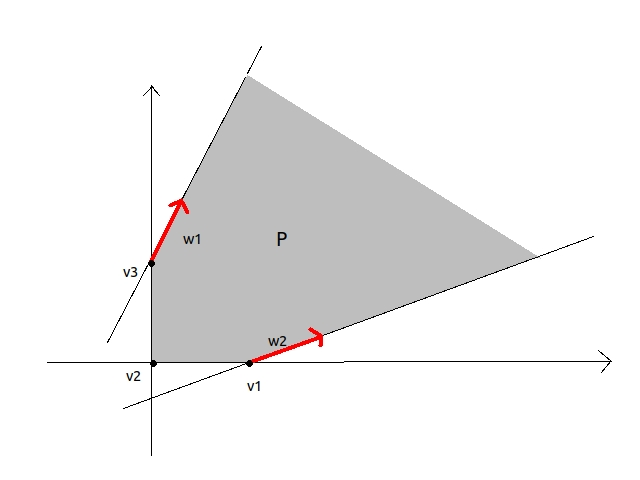
\includegraphics[width=0.7\textwidth]{Minkowski.jpg}
  \caption{Graphical example of Minkowskis representation Theorem}
  \label{fig:Bild1}
\end{figure}
\end{Teo}

So, every $x_i \in Q_i$ can be written as 
\begin{equation}
\label{eq:xMinkowski}
x_i = \sum_{j = 1}^{N_i} \lambda_{ij}v_{ij} + \sum_{l = 1}^{L_i} \mu_{il}w_{il}
\end{equation}

Recall that if $Q_i$ is bounded, the $\mu_{il}$ are 0 and you have a simpler notation. $N_i$ is the number of extreme points (or equivaltently, the number of vertices) of $Q_i$ and $L_i$ is the number of extreme rays of $Q_i$. Remember also that $n_i$ is the dimension of $Q_i$.


If we insert now \eqref{eq:xMinkowski} into \eqref{eq:particularFormDantzig}, we obtain a different but equivalent LP problem, called the \textit{master problem},
\begin{equation}
\begin{aligned}  
\min \enspace &\sum_{i = 1}^m  \left(\sum_{j=1}^{N_i}  \lambda_{ij}(c_i^Tv_{ij}) + 
	\sum_{l=1}^{L_i} \mu_{il}(c_i^Tw_{il}) \right) \\
\text{s.t.} \enspace &\sum_{i = 1}^m \left(\sum_{j=1}^{N_i}  \lambda_{ij}(A_{0i}v_{ij}) + 	\sum_{l=1}^{L_i} \mu_{il}(A_{0i}w_{il}) \right) = b_0 \\
&\sum_{j = 1}^{N_i} \lambda_{ij} = 1 \quad \forall i = 1,\dots ,m \\
&\lambda_{ij}, \mu_{ij} \geq 0 \quad \forall i,j
\label{eq:DantzigMaster}
\end{aligned}
\end{equation}
where the second kind of constraints follow from the fact that if $x_i$ satisfies  $A_{ii}x_i \leq b_i$, which means that $x_i \in Q_i$, then by the Minkowski representation Theorem, $x_i$ is convex combination of the $\lambda_{ij}$ (therefore this constraints) plus a combination of the $\mu_{il}$ (no particular constraints for this variables).


We can observe the following things:
\begin{itemize}
\item This problem \eqref{eq:DantzigMaster} is equivalent to the original problem \eqref{eq:particularFormDantzig}.
\item We have now other decision variables: The new ones are the weights of the extreme
points $(\lambda_{ij})$, and the weights of the extreme rays $(\mu_{ij})$.
\item The number of decision variables is now huge, much more than in the original formulation. To deal with this new big amount of variables, to solve the problem we will use the \textit{Revised Simplex Method}, which ignores a great part of them. The next sections explain this method and the final algorithm to solve problem \eqref{eq:DantzigMaster}. 
\item But in contrast, the number of constraints is smaller: The original problem has $\sum_{i =0}^m k_i$ constraints, while the new formulation has only $k_0 + m$ constraints, since the block constraints $A_{ii}x_i \leq b_i$ of $k_i$ constraints are now replaced by the single constraint $\sum_{j=1}^{N_i} \lambda_{ij} = 1$. 
\end{itemize}


\subsection{Revised Simplex Algorithm}
\label{chapter:RevisedSimplex}

A disadvantage of the Simplex Algorithm is that if you have a lot of variables and constraints, at every step you have to update the entire tableau. But to improve your solution with the simplex method you need only one negative reduced cost. The revised simplex method eliminates this disadvantage. 

Consider the standard minimum problem \eqref{eq:standard_minimum_lp}, and introduce slack variables to obtain the following form:

\begin{equation}
\begin{aligned}  
\min \enspace& c^Tx \\
\text{s.t.} \enspace& Ax = b \\
&x_j \geq 0 \quad \forall j 
\label{eq:standRevised}
\end{aligned} 
\end{equation}

Observe that \eqref{eq:DantzigMaster} is in this form.

We obtain a matrix $A \in \mathbb{R}^{n \times m}$ with $m \gg n$. So we can write $A = (B,R)$\footnote{$B$ doesn't have to be the first columns of $A$, but any set of columns can be taken, but then $c,b$ and $x$ need to be reordered.} where $B$ is a basis of $A$, i.e. a square and invertible matrix. We write also $x = (x_B,x_R)$. Now, since $Ax = b$, we have
\begin{align*}
Bx_B +Rx_R &= b \\
Bx_B &= b - Rx_R \\
x_B &= B^{-1}b - B^{-1}Rx_R
\end{align*}   

Thus we have expressed $x_B$ in function of $x_R$. To deal with less variables, we let all $x_i \in x_R$ be $0$. So our initial solution, a basic solution, is
\[
x_B = B^{-1}b,
\]
which of course has to be greater than zero to be a feasible solution.

Now we split also the cost vector $c$ in $(c_B,c_R)$, and we want to minimize $c^Tx$. Using the two previous results, it follows that
\begin{align*}
c^Tx &= c_Bx_B + c_Rx_R \\
&= c_B( B^{-1}b - B^{-1}Rx_R) + c_Rx_R \\
&= c_BB^{-1}b + (c_R-c_BB^{-1}R)x_R 
\end{align*}

So we get an optimality condition: since we are minimizing  and all decision variables $x_i$ have to be greater than $0$, we have an optimal solution if the vector $c_R-c_BB^{-1}R$ is positive since we set all non basis variables $x_R = 0$. If there is a negative entry we have to update the basis\footnote{For the scope of this paper it is not important how to update the basis in general.}. The coefficient of $x_j$ in $(c_R-c_BB^{-1}R)x_R$ is $d_j := c_j - c_BB^{-1}a_j$ where $a_j$ is the $j^{th}$ column of matrix $A$. $d_j$ is called the reduced cost of variable $x_j$. 

Therefore, problem \eqref{eq:standRevised} is solved by applying the simplex method iteratively to the much smaller problem 

\begin{equation}
\begin{aligned}  
\min \enspace& c_B^Tx_B \\
\text{s.t.} \enspace& Bx_B = b_B \\
&x_B \geq 0 
\label{eq:Revisedprimal}
\end{aligned}
\end{equation}

where you have to update the basis at every step to find the optimal basis. To check that $(x_B,0)$ is optimal for \eqref{eq:standRevised}, you have to check that $d_j>0 \enspace \forall j$. To simplify the calculations of $d_j$, let $y^T := c_B^TB^{-1}$. You can see that $y$ are the dual variables of \eqref{eq:Revisedprimal}, thus if we solve \eqref{eq:Revisedprimal} with the simplex method, it gives us as output $x_B$, but also $y$. So 
\begin{equation}
\label{eq:reduced cost}
d_j = c_j - y^Ta_j
\end{equation}



\subsection{Algorithm}

Now we have all ingredients to solve \eqref{eq:DantzigMaster}. The revised simplex method turns out to be useful for this aim since we have much more variables than constraints. 

To start we need a basis. There is no particular rule which basis (or equivalently, which vertices or extreme rays) to take. The only constraint is that the inital basic solution you choose has to be feasible, take care about this! This beginning problem with a reduced number of variables is called the \textit{restricted master problem} which is solved with the simplex method, where we denote the optimal vector by $\widehat{x}$.

To check if the output from the restricted master problem is also optimal for the entire problem (if you are lucky and choose directly the optimal basis), you have to calculate the reduced cost $\overline{\lambda_{ij}}$ of variable $\lambda_{ij}$ and the reduced cost $\overline{\mu_{il}}$ of variable $\mu_{il}$ via the formula given by \eqref{eq:reduced cost} and you have to check if they are non negative. By solving the restricted master problem we get from the simplex method not only $\widehat{x}$, but also the vector $y$, the dual variables form the coupling constraints and the vector $z$, the dual variables from the simple constraints. In the notation of \eqref{eq:DantzigMaster}, \eqref{eq:reduced cost} becomes



\begin{equation}
\label{eq:reducedCostlDantzig}
\begin{aligned}
\overline{\lambda_{ij}} &= c_i^Tv_{ij} - ((A_{0i}v_{ij})^Ty+e_i^Tz) \\
 &= c_i^Tv_{ij} - (A_{0i}v_{ij})^Ty - z_i \\
 &= (c_i - A_{0i}^Ty)^Tv_{ij} - z_i
\end{aligned}
\end{equation}

\begin{equation}
\label{eq:reducedCostmDantzig}
\begin{aligned}
\overline{\mu_{il}} &= c_i^Tw_{il} - ((A_{0i}w_{il})^T) \\
 &= c_i^Tw_{il} - (A_{0i}w_{il})^Ty  \\
 &= (c_i - A_{0i}^Ty)^Tw_{il} 
\end{aligned}
\end{equation}

But calculating every reduced cost would be an enormous work since we have a lot of variables. So instead of calculating for every variable the reduced cost, we solve the following $m$~subproblems:

\begin{equation}
\begin{aligned}
\min \enspace &(c_i - A_{0i}^Ty)^Tx \\
\text{s.t.} \enspace &A_{ii} = b_i \\
 & \quad x \geq 0
\end{aligned}
\label{eq:subproblem}
\end{equation}

It can be done in this way since the reduced costs are equal or similar to the form $(c_i - A_{0i}^Ty)^Tx$, where $x$ is or $v_{ij}$ or $w_{il}$. Since the simplex method gives as output of this $i^{th}$ subproblem a vertex or extreme ray of $Q_i$, we can find for every subproblem the smallest reduced cost. 

So, the optimal solution of this $i^{th}$ subproblem is or a vertex $v_{ik}$, if the objective function value is bounded, or an extreme ray $w_{ik}$, if the objective function value    is $-\infty$, of the set $Q_i$.  



Therefore, we have three possibilities:
\begin{itemize}
\item[1.] The objective function value is $-\infty$:
\begin{itemize}
\item Simplex output: an extreme ray $w_{ik}$  with $ (c_i - A_{0i}^Ty)^Tw_{ik}  < 0$
\item Conclusion: the reduced cost $\overline{\mu_{ik}}$ of $\mu_{ik}$ is negative.
\item Action: introduce the variable $\mu_{ik}$ in the restricted master problem.
\end{itemize}
\item[2.] The objective function value is finite, but less then $z_i$:
\begin{itemize}
\item Simplex output: extreme point $v_{ik}$ with $ (c_i - A_{0i}^Ty)^Tv_{ij} < z_i $
\item Conclusion: the reduced cost $\overline{\lambda_{ik}}$ of $\lambda_{ik}$ is negative.
\item Action: introduce the variable $\lambda_{ik}$ in the restricted master problem.
\end{itemize}
\item[3.] The objective function value is finite and bigger or equal then $z_i$:
\begin{itemize}
\item Conclusion: $ (c_i - A_{0i}^Ty)^Tv_{ij} \geq z_i $ for all extreme points $v_{ik}$ and $ (c_i - A_{0i}^Ty)^Tw_{ik}  \geq 0$ for all extreme rays $w_{ik}$
\item Action: Terminate, you have found an optimal basis since all reduced costs are non negative.
\end{itemize}
\end{itemize}

\paragraph*{Summary}

\begin{itemize}
\item[0.] Find an initial basic feasible solution (take care about this, see chapter \ref{chapter:RevisedSimplex}) and create the initial restricted master problem. 
\item[1.] Solve the restricted master problem (with the simplex method), and store the dual variables $y$ and $z$.
\item[2.] Solve the $m$ subproblems.
If the optimal cost of subproblem $i$ is bigger or equal than $z_i$ (case 3), terminate with optimal solution \eqref{eq:xMinkowski} where the $\lambda_{ij}$ and $\mu_{ij}$ are the solutions of the restricted master problem.
\item[3.] If subproblem $i$ is unbounded, add variable $\mu_{il}$ to the restricted master problem.
\item[4.] If subproblem $i$ has bounded optimal cost less than $z_i$, add variable $\lambda_{ij}$ to the restricted master problem.
\item[5.] Generate a column associated with the entering variable and continue with step one. 
\end{itemize}

\newpage

\subsection{Bounds}

Let us think about upper and lower bounds for this method. Let $s^\star$ be the  best value for the objective function, i.e. $s^\star = c^Tx^\star$ where $x^\star$ is the optimal vector of problem \eqref{eq:particularFormDantzig}.

\paragraph*{Upper bound}

It is easy to see, that the solution given by the restricted master problem is an upper bound of the master problem, since it is a feasible solution of the problem. 

\paragraph*{Lower bound}

To deduce a lower bound, we use the dual maximization problem, i.e. \eqref{eq:cx<yb}.
Now, the dual problem of the master problem \eqref{eq:DantzigMaster} would be

\begin{equation}
\begin{aligned}
\label{eq:DantzigMasterDual}
\max \enspace  & y^Tb_0 + z_1 + z_2 + \dots + z_m  \\
\text{s.t.} \enspace & y^TA_{0i}v_{ij} + z_i \leq c_i^Tv_{ij} \enspace \quad \forall i, \forall j \in N_i \\
& y^TA_{0i}w_{il} \leq c_i^Tw_{il} \quad \quad \: \forall i, \forall l \in L_i .
\end{aligned}
\end{equation}

Let  $s_i$ the optimal objective function value for every subproblem $i$ and $\overline{y}, \overline{z}$ be the optimal dual vectors for the restricted master problem. We have that, if $s_i$ is bounded, by \eqref{eq:subproblem}, that

\begin{align*}
s_i \leq\: & c_i^Tv_{ij} - \overline{y}^TA_{0i}v_{ij} \quad \forall j \in N_i \\
  0 \leq\: & c_i^Tw_{il} - \overline{y}^TA_{0i}w_{il} \quad \forall l \in L_i
\end{align*} 

It follows that $\overline{y}$ and the $s_i$ are feasible solutions of \eqref{eq:DantzigMasterDual}, but not necessary optimal solutions. Therefore we have

\[
s^\star \geq \overline{y}^Tb_0 + s_1 + s_2 + \dots + s_m
\]

Let now $s$ be the optimal objective function value for the restricted master problem. We use \eqref{DualityTheorem} again to deduce that $s = \overline{y}^Tb_0 + \overline{z_1} + \dots + \overline{z_m}$. Plug this result in the above equation and you obtain a lower bound:

\begin{equation}
s^\star \geq s + (s_1 - \overline{z_1}) + (s_2 - \overline{z_2}) + \dots + (s_m - \overline{z_m})
\end{equation}

So, we have that 
\[
s + (s_1 - \overline{z_1}) + (s_2 - \overline{z_2}) + \dots + (s_m - \overline{z_m}) \leq s^\star \leq s
\]


\subsection{Examples}

Now let us do some small numerical examples to understand the procedure better.

\paragraph*{Example 1}

\begin{align}
\min \enspace &  -4x_1 - x_2 - 6x_3  \label{eq:ex1objective}\\
\text{s.t.} \enspace & 3x_1 + 2x_2 + 4x_3 = 17 \label{eq:ex1couplecon} \\
& 1 \leq x_1  \leq 2 \label{eq:ex1con1}\\ 
& 1 \leq x_2  \leq 2 \label{eq:ex1con2}\\
& 1 \leq x_3  \leq 2 \label{eq:ex1con3}
\end{align}

The last constraints \eqref{eq:ex1con1} - \eqref{eq:ex1con3} tell us that the constraint set is bounded, so all weights $\mu_{ij}$ of the extreme rays $w_{ij}$ are zero. Now we have to choose which constraint is the coupling constraint and which are the other constraints, i.e. the matrices $A_{0i}$ and $A_{ii}$. We decide to let $m = 1$, $A_{01} = [3 \enspace 2 \enspace 4]$, $b_0 = 17$, $c^T = [-4 \enspace -1 \enspace -6]$ and the set $Q_1$ be defined by constraint \eqref{eq:ex1con1}, \eqref{eq:ex1con2}, \eqref{eq:ex1con3}. So $Q_i$ is a cube with 8 vertices. As explained before, we don't want to introduce all 8 vertices as new variables, so we start by choosing an admissible basis. We pick the vertices $v_1^T = (2,2,2)$ and $v_2^T = (1,1,2)$, which are feasible vertices (see chapter \ref{chapter:RevisedSimplex} to determine how many vertices you need and to verify if these two vertices are feasible).

\begin{figure}[htbp] 
  \centering
     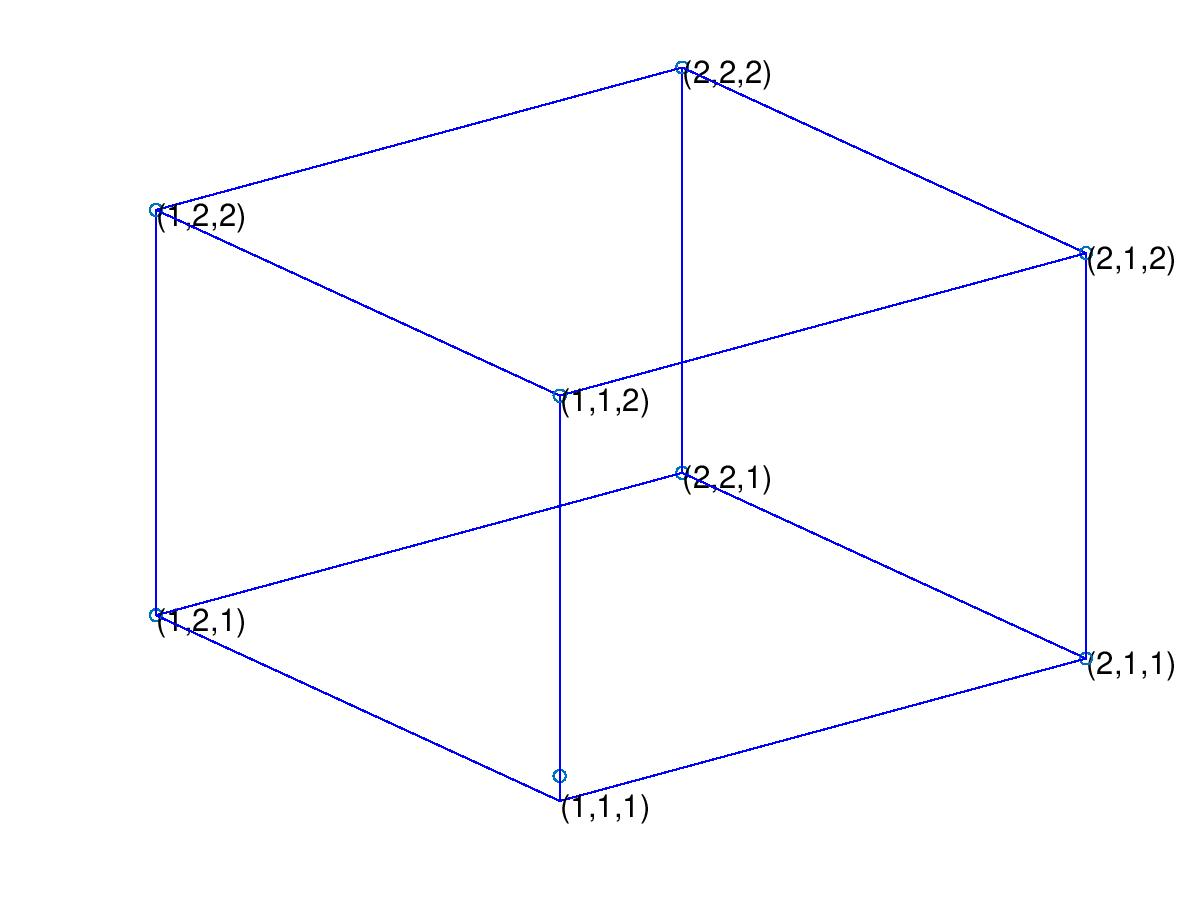
\includegraphics[width=0.5\textwidth]{cube.jpg}
  %\caption{Cube $Q_i$}
\end{figure}


 Now we can transform our original problem into the restricted master problem:


\begin{align*}
\min \enspace & (c_{1}^Tv_1)\lambda_1  + (c_{1}^Tv_2)\lambda_2 \\
\text{s.t.} \enspace & (A_{01}v_1)\lambda_1 + (A_{01}v_2)\lambda_2 = 17 \\
& \lambda_1 + \lambda_2 = 1 \\
& \lambda_1 , \lambda_2 \geq 0
\end{align*}


which becomes 


\begin{align*}
\min \enspace & -22\lambda_1  - 17\lambda_2 \\
\text{s.t.} \enspace & 18\lambda_1 + 13\lambda_2 = 17 \\
& \lambda_1 + \lambda_2 = 1 \\
& \lambda_1 , \lambda_2 \geq 0
\end{align*}

We solve this problem now with the simplex method, and we get as optimal vector $\lambda = (\lambda_1, \lambda_2) = (0.8,0.2)$, and optimal dual vector $t = (y,z) = (-1,-4)$. (You can check this result, since by \eqref{eq:optimality}, $-21 = c^T\lambda = tb^T = -21.$)

Now we have to solve the subproblems. In this case, since $m=1$, we have only one subproblem with coefficients given by $c^T - y^TA_{01}:$

\[
[-4 \enspace -1 \enspace -6] - (-1) [3 \enspace 2 \enspace 4] = [-1 \enspace 1 \enspace -2].
\]

So the subproblem is
\begin{align*}
\min \enspace &  -x_1 + x_2 - 2x_3  \\
& 1 \leq x_1  \leq 2 \\ 
& 1 \leq x_2  \leq 2 \\
& 1 \leq x_3  \leq 2 
\end{align*}

The optimal vector of this subproblem is $v_3^T = (2,1,2)$ with objective function value $s_1 = -5$ which is smaller than $z = -4$. Thus we introduce $v_3$ in the basis. Now we update the restricted master problem, inserting variable $\lambda_3$ which correspondents to vertex $v_3$. The restricted master problem becomes

\begin{align*}
\min \enspace & -22\lambda_1  - 17\lambda_2 - 21\lambda_3 \\
\text{s.t.} \enspace & 18\lambda_1 + 13\lambda_2 + 16\lambda_3 = 17 \\
& \lambda_1 + \lambda_2 +\lambda_3 = 1 \\
& \lambda_1 , \lambda_2, \lambda_3 \geq 0
\end{align*}

The optimal vector is $\lambda_1 = 0.5$, $\lambda_3 = 0.5$ with dual $y = -0.5$ and $z = -13$.

Now again we have to solve the new subproblem:

\[
[-4 \enspace -1 \enspace -6] - (-0.5) [3 \enspace 2 \enspace 4] = [-2.5 \enspace 0 \enspace -4].
\]

\begin{align*}
\min \enspace &  -2.5x_1  - 4x_3  \\
& 1 \leq x_1  \leq 2 \\ 
& 1 \leq x_2  \leq 2 \\
& 1 \leq x_3  \leq 2 
\end{align*}

The optimal vector of it is $v_4 = (2,2,2)$ with objective function value $s_1 = -13$, so we stop here since $z = -13$, and the optimal vector of example 1 is
\[
 x = 0.5v_1+0.5v_3 = [2 \enspace 1.5 \enspace 2]^T
\]

with optimal objective function value $s^\star = -21.5$. Note, that at the first iteration, if we look at the bounds, 
\[
-22 = -21 + (-5-(-4))= s + (s_1 - \overline{z_1})  \leq s^\star \leq s = -21
\]
Let's do now another example, with an unbounded constraint set.

\paragraph*{Example 2}

\begin{align*}
\min \enspace & -5x_1 + x_2 \\
\text{s.t.} \enspace & x_1 \leq 8 \\
& x_1 - x_2 \leq 4 \\
& 2x_1 - x_2 \leq 10 \\
& x_1 , x_2 \leq 0
\end{align*}

This problem is not in the form to solve it, i.e. we have no equality constraint which we can use as the coupling constraint. Therefore we introduce a slack variable $x_3$ to overcome this obstacle:

\begin{align}
\min \enspace & -5x_1 + x_2 \\
\text{s.t.} \enspace & x_1 + x_3 = 8 \\
& x_1 - x_2 \leq 4 \label{eq:ex2con1}\\
& 2x_1 - x_2 \leq 10 \label{eq:ex2con2}\\
& x_1 , x_2 , x_3 \leq 0
\end{align}

As you can see, we have now three variables. Moreover, you can divide the constraints in two pieces with independent variables: The first part would be constraint \eqref{eq:ex2con1}, \eqref{eq:ex2con2} and the nonnegativity constraints $x_1, x_2 \geq 0$. The second part would be only the constraint $x_3 \geq 0$. So we have two sets of independent variables, $Q_1$ and $Q_2$. By analyising these two sets, you can figure out that $Q_1$ has three extreme points, $v_{11} = (6,2), v_{12} = (4,0)$ and $v_{13} = (0,0)$, and two extreme rays, $w_{11} = (1,2)$ and $w_{12} = (0,1)$. $Q_2$ has simply one extreme ray $w_{21} = 1$. So in total, if we would transform the problem with these new variables, we would have six variables and two constraints.

\begin{figure}[htbp] 
  \centering
     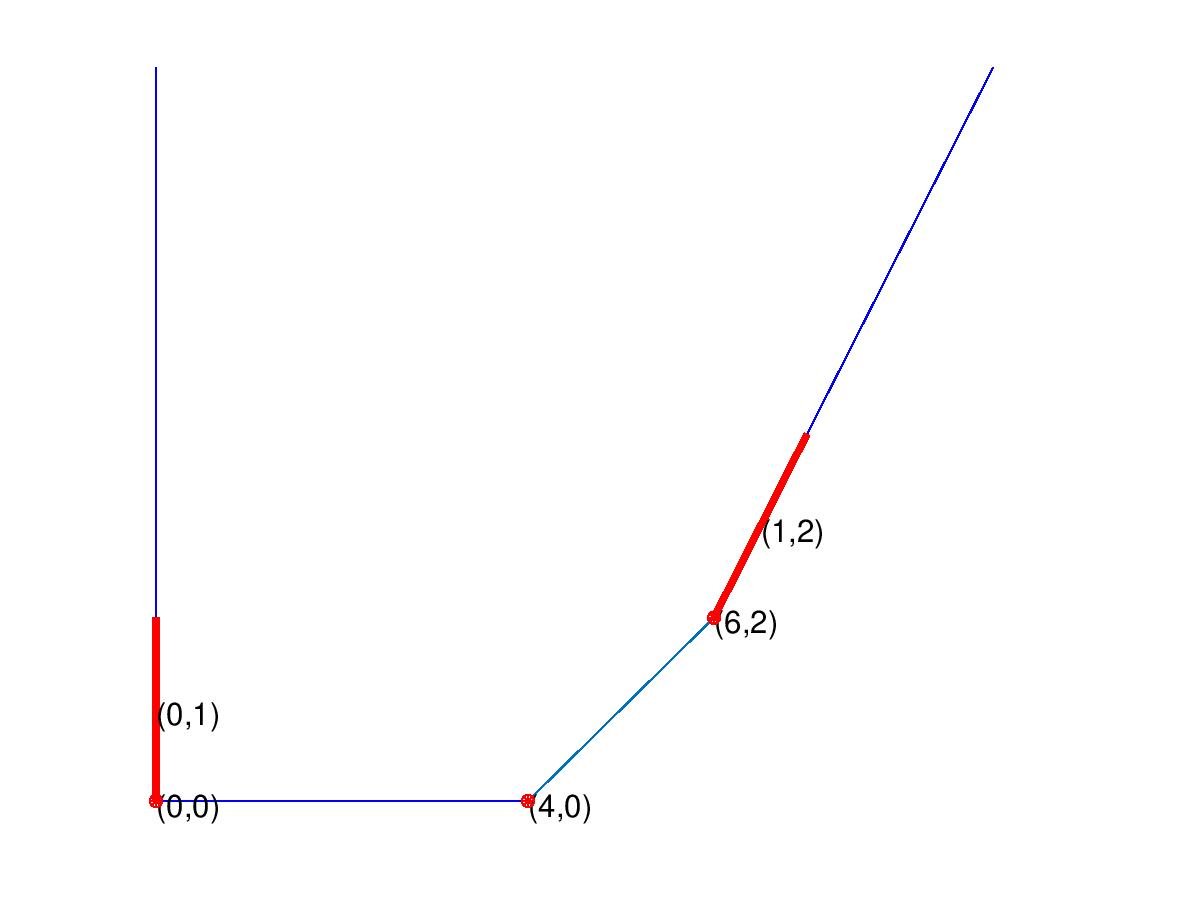
\includegraphics[width=0.5\textwidth]{q2.jpg}
  \caption{Set $Q_1$, as you can see it is unbounded.}
\end{figure}


Now we have to take an initial basis. We decide to take the extreme point $v_{11}$ and the extreme ray $w_{21}$. We transform the problem into the restricted master problem where you calcluate the coeficients in the same way as in the last example:

\begin{align*}
\min \enspace & -28\lambda_{11} \\
\text{s.t.} \enspace & 6\lambda_{11} + \mu_{21} = 8 \\
& \lambda_{11} = 1 \\
&\lambda_{11} , \mu_{21} \geq 0
\end{align*}

If we solve this problem with the simplex method, we obtain the optimal vector with $\lambda_{11} = 1, \mu_{21} = 2$ and with the optimal duals $y = 0$ and $z = -28$.

Again, now we have to calculate the coefficients for the subproblems: 

For subproblem 1, we have $c_1^T - y^TA _{01} = [ -5 \enspace 1] - (0)[1 \enspace 0] = [ -5 \enspace 1]$, and for subproblem 2 we have  $c_2^T - y^TA _{02} = 0 - (0)(1) = 0$. Therefore, we have only to solve subproblem 1 because subproblem 2 is trivial and gives a non negative reduced cost. Therefore, for subproblem 2 we know that we don't have to introduce a variable (This can also be obtained in a different way: Since we used all variables we have for representing $Q_2$, we can't improve the solution because we can not substract something since we don't have other variables.)

Thus, subproblem 1 is:

\begin{align*}
\min \enspace & -5x_1 + x_2 \\
& x_1 - x_2 \leq 4 \\
& 2x_1 - x_2 \leq 10 \\
& x_1 , x_2 \leq 0
\end{align*}

If we solve it with the simplex algorithm, we obtain as optimal vector the extreme ray $w_{11}  = (1,2)$ with objective function value $-\infty$. So we add variable $\mu_{11}$ to the restricted master problem, and we obtain:

\begin{align*}
\min \enspace & -28\lambda_{11} -3\mu_{11} \\
\text{s.t.} \enspace & 6\lambda_{11} + \mu_{21} + \mu_{11} = 8 \\
& \lambda_{11} = 1 \\
&\lambda_{11} , \mu_{21} , \mu_{11} \geq 0
\end{align*}

The simplex algorithm gives us the optimal vector with $\lambda_{11} =  1, \mu_{11} = 2$ and $\mu_{21} = 0$ with optimal duals $y = -3, z = -10$.

Again, to check optimality we have to check the reduced costs and therefore we have to solve subproblem 1, i.e.

\begin{align*}
\min \enspace & -2x_1 + x_2 \\
& x_1 - x_2 \leq 4 \\
& 2x_1 - x_2 \leq 10 \\
& x_1 , x_2 \leq 0.
\end{align*}

The value objective function of the optimal vector $(8,6)$ is $s_1 = -10$, which is (greater or) equal than $z$, thus the optimal solution of example 2 is

\[
x = v_{11} + 2w_{11} = [8 \enspace 6]^T.
\]

\subsection{Dantzig-Wolfe in ILP}

Consider the integer linear programming problem

\begin{equation}
\begin{aligned}
s^\star =&\min \{c^Tx: x \in X\} \\
X =& Y \cap Z \\
Y =& \{x: Dx \geq d\} \\
Z =& \{x: Bx \geq b\} \cap \mathbb{Z}^n_+
\end{aligned}
\label{eq:ILPDantzig}
\end{equation}

The idea to solve this with the Dantzig-Wolfe method is, to use the Minkowski representation Theorem for $conv(Z)$, i.e for the convex hull of $Z$.

If we reformulate it with the new variables, we get

\begin{align*}
s^{\star} &= \min_{\lambda \geq 0} \sum_{j = 1}^J (c^Tv_j)\lambda_j \\
\text{s.t.} \enspace & \sum_{j = 1}^J (Dv_j)\lambda_j \geq d \\
&\sum_{j = 1}^J \lambda_j = 1 \\
&\sum_{j = 1}^J v_j \lambda_j \in \mathbb{Z}^n 
\end{align*}

where the $v_j$ are the vertices of $conv(Z)$ and $J$ is the number of vertices of $conv(Z)$. This is called the \textit{master problem.}

As before, to solve it we define the restricted master problem to deal with less variables at once. Thus, the restricted master problem is 

\begin{align*}
s^{DWrestricted} = \min_{\lambda \geq 0} \enspace & \sum_{j = 1}^{\overline{J}} (c^Tv_j)\lambda_j \\
\text{s.t.} \enspace & \sum_{j = 1}^{\overline{J}} (Dv_j)\lambda_j \geq d \\
&\sum_{j = 1}^{\overline{J}} \lambda_j = 1 
\end{align*}

where $\overline{J} \subset J$. Let $y$ be the dual variable of the first constraint and $z$ be the dual variable of the second constraint of the restricted master problem.

As in the Dantzig-Wolfe algorithm in LP, to check optimality we need the reduced cost for every variable $\lambda_j$, and it is again $c^T v_j - y^T Dv_j - t$. So, if we use the same trick to avoid to calculate all reduced costs, 

\begin{equation}
\min_{Bx\geq b,x\in Z^n_+} (c^T - y^TD)x
\label{eq:ILPsubproblem}
\end{equation}

has to be an easy ILP problem which we can solve quickly. Moreover, as in the LP case, we can deduce the same bounds, i.e. the solution of the restricted master problem is an upper bound for the master problem and $y^T d + s$ a lower bound.

Thus, to solve \eqref{eq:ILPDantzig} we do the following steps:

\begin{itemize}
\item[1.] Inizialize the upper bound $UB = +\infty$ and the lower bound $LB = -\infty$.
\item[2.] Find an initial basis $v_1$ and $v_2$ and Let $\overline{J} = \{v_1,v_2\}$.
\item[3.] Compute the restricted master problem with $\overline{J}$
\begin{itemize}
\item[a.] Solve the restricted master problem. Store its solution, the optimal dual vector $(y,z)$ and update $UB$.
\item[b.] Solve the subproblem $s = \min\{(c^T - y^TD)x : x \in Z \}$ and let $v_k$ be the optimal vector. If $z = s$, stop the algorithm with optimal solution given by the restricted master problem, else add $v_k$ to $\overline{J}$.
\item[c.] Update the lower bound: $LB  = \max\{LB,y^T d + s\}$. If $LB = UB$, stop the algorithm with optimal solution given by the restricted master problem.
\item[d.] Repeat step 3.
\end{itemize}
\end{itemize}

But, anyway, if \eqref{eq:ILPsubproblem} is not easy to solve, this method is useless. In fact, the Dantzig-Wolfe decomposition is not that much used for ILP problems, because you don't know a priori if \eqref{eq:ILPsubproblem} is easy to solve or not.

\newpage

\section{AMPL code}

\subsection{The mod file}
\begin{lstlisting}
# DANTZIG-WOLFE DECOMPOSITION
# Bounded Problem

param N; #total number of variables     DATA
param K; #total number of constraints   DATA
param m; #number of systems             DATA 

param ni{1..m}; #subdivision of variables, nj[j] = dimension;               DATA
param ki{0..m}; #subdivision of constraints in sets of ki[i] constraints;   DATA

#only two checks if parameters are set up in the right way
check: sum{j in 1..m} ni[j] = N;
check: sum{i in 0..m} ki[i] = K; 



param b{i in 0..m,1..ki[i]}; #all constraint values, subdivised          DATA
param c{i in 1..m,1..ni[i]}; #all cost values, subdivised                DATA

set index = {0..m,1..m}; #index (i,j) of matrices A[i,j] 
set iindex within index; #specify what matrices   DATA

param A{(i,j) in iindex, 1..ki[i], 1..ni[j]};#Matrices A[i,j] DATA

#cost of subproblem m
param cost_subproblem{1..m,1..ni[m]};  #        RUN
#to calculate it, you need the following:
#dual variable y (of coupling constraints)
param dual_cost_y{1..ki[0]}; #                  RUN
#dual variabls z (of simple constraints)
param dual_cost_z{1..m}; #                      RUN

var x{p in 1..m, 1..ni[p]} >= 0;   


# THE m SUBPROBLEMS:

minimize Reduced_Cost{p in 1..m}:
   sum{i in 1..ni[p]} cost_subproblem[p,i]*x[p,i];


subject to Set_constraint{p in 1..m,j in 1..ki[p]}:
	sum{i in 1..ni[p]} A[p,p,j,i]*x[p,i] <= b[p,j];



# RESTRICTED MASTER PROBLEM 




#number of vertices of set Q(i) (subproblem i), 
param numberOfvertices{1..m} integer >= 0;  #                     RUN
#changes during execution, 


#vertices values to corresponding lambdas, 
#introduced with the RUN file
param vertices{p in 1..m, 1..numberOfvertices[p], 1..ni[p]}; #    RUN

param numberOfInitialVertices{p in 1..m}; #DATA
param initial_vertices{p in 1..m, 1..numberOfvertices[p], 1..ni[p]}; #DATA





#c_i*v_ik
param restricted_master_cost{p in 1..m, 1..numberOfvertices[p]};# RUN

param restricted_couple_cost{p in 1..m, 1..numberOfvertices[p], 1..ki[0]};#RUN


var lambda{p in 1..m, 1..numberOfvertices[p]} >= 0;


minimize Total_Restricted_Cost:
   sum{p in 1..m, k in 1..numberOfvertices[p]} 
      restricted_master_cost[p,k]*lambda[p,k];

subject to Restricted_Coupled {j in 1..ki[0]}:
	sum{p in 1..m, k in  1..numberOfvertices[p]} 
		restricted_couple_cost[p,k,j]*lambda[p,k] = b[0,j];
      

subject to Convex{p in 1..m}: 
	sum{k in 1..numberOfvertices[p]} lambda[p,k] = 1;


#to check if the initial values are admissible



#
#var y{1..m,1..ki[0]}; 

#nothing to maximize, only to check if B^-1*b>=0
#
#maximize nothing: 0;

#
#subject to couple{i in 1..ki[0]}:
#	sum{p in 1..m, j in 1..numberOfvertices[p]}
#		restricted_couple_cost[p,j,i]*y[p,j] = b[0,i];
		
#subject to convex2{p in 1..m}:
#	sum{i in 1..numberOfvertices[p]} y[p,i] = 1;



\end{lstlisting}


\subsection{The run file}
\begin{lstlisting}
# DANTZIG-WOLFE DECOMPOSITION 
# on bounded sets


model DWgeneral.mod;
data DWgeneral.dat;

param nIter default 0;
param success default 0;
param mincost;
param initialChekparameter default 0;
#option omit_zero_rows 1;
#option display_1col 0;
option display_eps .000001;

# ----------------------------------------------------------

#Restricted Master
problem RMaster: Total_Restricted_Cost, lambda, Restricted_Coupled, Convex;

#Subproblems
problem Subproblem{p in 1..m}: 
	Reduced_Cost[p], 
	{j in 1..ni[p]} x[p,j],
	{i in 1..ki[p]} Set_constraint[p,i]; 


#to check if initial data is feasible
#problem initialCheck: nothing, y, couple, convex2;



let {i in 1..ki[0]} dual_cost_y[i] := 1;
let {p in 1..m} dual_cost_z[p] := 1;
let {p in 1..m} numberOfvertices[p] := numberOfInitialVertices[p];

let {p in 1..m, i in 1..ni[p]} cost_subproblem[p,i] := 
		c[p,i] - (sum{j in 1..ki[0]} dual_cost_y[j]*A[0,p,j,i]);

let{p in 1..m,i in 1..numberOfvertices[p],j in 1..ni[p]}
	 vertices[p,i,j] := initial_vertices[p,i,j];




#At the beginning step we need the costs for the RM:
let {p in 1..m,i in 1..numberOfvertices[p]}
	restricted_master_cost[p,i] := sum{j in 1..ni[p]} c[p,j]*vertices[p,i,j];




	

let {p in 1..m,j in 1..ki[0], k in 1..numberOfvertices[p]}
	restricted_couple_cost[p,k,j] :=
		sum{i in 1..ni[p]} A[0,p,j,i]*vertices[p,k,i];

#a check if you have the right amount of beginning variables (not necessary?)
if sum{p in 1..m} numberOfvertices[p] < ki[0] + m then {
	printf "\nNOT EXACT NUMBER OF INITIAL VECTORS.\n";
	};


####ONLY CHEK, NOT NECESSARY
#solve initialCheck;

#for {p in 1..m} {
#	for {j in 1..numberOfvertices[p]} {
#		if y[p,j] >= 0 then {
#			let initialChekparameter := initialChekparameter + 1;
#		}
#	}
#}

#if initialChekparameter < ki[0]+m then {
#	printf "\nNO CORRECT INITIAL DATA! POSSIBLY WRONG OUTPUT.\n";
#}

####CHECK UP TO HERE

repeat { 

	let nIter := nIter + 1;
	printf "\nITERATION %d\n", nIter;
	
	#let {p in 1..m,j in 1..ki[0], k in 1..numberOfvertices[p]}
	#restricted_couple_cost[p,k,j] :=
	#	sum{i in 1..ni[p]} A[0,p,j,i]*vertices[p,k,i];
	
	display restricted_master_cost;
	display restricted_couple_cost; 
	solve RMaster;
	
	printf "\nRestrictedMaster solution nr. %d\n", nIter;
	display lambda;
	
	let {i in 1..ki[0]} dual_cost_y[i] := Restricted_Coupled[i].dual;#lambda dual Restricted_Couple;
	let {p in 1..m} dual_cost_z[p] := Convex[p].dual;#lambda dual convex
	
	printf "\nDual variables nr. %d\n", nIter;
	display dual_cost_z;
	display dual_cost_y;
	
	let {p in 1..m,i in 1..ni[p]} cost_subproblem[p,i] := 
		c[p,i] - (sum{j in 1..ki[0]} dual_cost_y[j]*A[0,p,j,i]);
	
	display cost_subproblem;

	
	for {p in 1..m} { 

		solve Subproblem[p];

		if Reduced_Cost[p] < dual_cost_z[p] -0.00001 then {
			printf "\nNew vertex of supbroblem %d\n", p;
			display {i in 1..ni[p]} x[p,i];	
			let numberOfvertices[p] := numberOfvertices[p] + 1;
			let{i in 1..ni[p]} vertices[p, numberOfvertices[p], i] := x[p,i];
			let restricted_master_cost[p,numberOfvertices[p]] :=
				sum{j in 1..ni[p]} c[p,j]*vertices[p,numberOfvertices[p],j];
		
			display restricted_master_cost;
		
		}
		
		else {
			let success := success+1;
		};
	};
	if success = m then {
		printf "\nOPTIMAL SOLUTION:\n";
		
		let {p in 1..m,i in 1..ni[p]} 
			x[p,i] := sum{j in  1..numberOfvertices[p]} 
				lambda[p,j]*vertices[p,j,i];
			display x;
			printf "\nOBJECTIVE FUNCTION VALUE:\n";
			let mincost := sum{p in 1..m,i in 1..ni[p]} x[p,i]*c[p,i];
			display mincost;
		break;
	};
	let success := 0;
	
	let {p in 1..m,j in 1..ki[0], k in 1..numberOfvertices[p]}
	restricted_couple_cost[p,k,j] :=
		sum{i in 1..ni[p]} A[0,p,j,i]*vertices[p,k,i];
};	

\end{lstlisting}

\newpage
\subsection{Examples for data files}

\subsubsection{Example 1}
\begin{lstlisting}

# DANTZIG-WOLFE DECOMPOSITION
# Bounded Problem

param N := 3; #total number of variables
param K := 7; #total number of constraints
param m := 1; #number of systems 

#subdivision of variables, nj[j] = dimension;
param ni :=
1 3;

#subdivision of constraints in sets of ki[i] constraints;
param ki :=
0 1
1 6; 

#all constraint values, subdivised
#b{i in 0..m,1..ki[i]}
param b :=
	[0,*] :=
		1 17
	[1,*] :=
		1 2
		2 2
		3 2
		4 -1
		5 -1
		6 -1;

#all cost values, subdivised 
#{i in 1..m,1..ni[i]}
param c :=
	[1,*] :=
		1 -4
		2 -1
		3 -6;
		
#within index; #specify what matrices, can done by RUN
set iindex := 
(0,1)
(1,1);

#{(i,j) in iindex, 1..ki[i], 1..ni[j]}
param A := 
	[0,1,*,*]: 1 2 3 :=
		1 3 2 4
	[1,1,*,*]: 1 2 3:=
		1 1 0 0
		2 0 1 0
		3 0 0 1
		4 -1 0 0
		5 0 -1 0
		6 0 0 -1;
		
		
param numberOfInitialVertices := #{p in 1..m};
1 2;

#{p in 1..m, 1..numberOfvertices[p], 1..ni[p]}; 		
param initial_vertices := 
		[1,*,*]: 1 2 3:=
			1 2 2 2
			2 1 1 2;
\end{lstlisting}

\newpage
\subsubsection{Example 2}
\begin{lstlisting}
# DANTZIG-WOLFE DECOMPOSITION
# Bounded Problem

param N := 5; #total number of variables
param K := 8; #total number of constraints
param m := 2; #number of systems 

#subdivision of variables, nj[j] = dimension;
param ni :=
1 2
2 3;

#subdivision of constraints in sets of ki[i] constraints;
param ki :=
0 2
1 2
2 4; 

#all constraint values, subdivised
#b{i in 0..m,1..ki[i]}
param b :=
	[0,*] :=
		1 4
		2 1
	[1,*] :=
		1 7
		2 8
	[2,*] :=   
		1 3
		2 7
		3 5
		4 3;

#all cost values, subdivised 
#{i in 1..m,1..ni[i]}
param c :=
	[1,*] :=
		1 -4
		2 -2
	[2,*] :=
		1 -2
		2 -4
		3 -1;
		
#within index; #specify what matrices, can done by RUN
set iindex := 
(0,1)
(0,2)
(1,1)
(2,2);

#{(i,j) in iindex, 1..ki[i], 1..ni[j]}
param A := 
	[0,1,*,*]: 1 2 :=
		1 1 2 
		2 1 2
	[0,2,*,*]: 1 2 3 := 
		1 3 2 -4
		2 -3 2 -1
	[1,1,*,*]: 1 2 :=
		1 4 2
		2 1 2
	[2,2,*,*]: 1 2 3 :=
		1 1 0 1
		2 2 3 1
		3 3 -1 1
		4 2 -1 1;
		
		
		
param numberOfInitialVertices := #{p in 1..m};
1 2
2 2;

#{p in 1..m, 1..numberOfvertices[p], 1..ni[p]}; 		
param initial_vertices := 
		[1,*,*]: 1 2 :=
			1 1 1.5
			2 1.75 0
		[2,*,*]: 1 2 3:=
			1 2 1 0
			2 0 1.33333333 3;
\end{lstlisting}
\newpage
\subsection{Output}

\subsubsection{Example 1}
\begin{lstlisting}
ITERATION 1
restricted_master_cost :=
1 1   -22
1 2   -17
;

restricted_couple_cost :=
1 1 1   18
1 2 1   13
;

MINOS 5.51: optimal solution found.
1 iterations, objective -21

RestrictedMaster solution nr. 1
lambda :=
1 1   0.8
1 2   0.2
;


Dual variables nr. 1
dual_cost_z [*] :=
1  -4
;

dual_cost_y [*] :=
1  -1
;

cost_subproblem :=
1 1   -1
1 2    1
1 3   -2
;

MINOS 5.51: optimal solution found.
2 iterations, objective -5

New vertex of supbroblem 1
x[p,i] [*] :=
1  2
2  1
3  2
;

restricted_master_cost :=
1 1   -22
1 2   -17
1 3   -21
;


ITERATION 2
restricted_master_cost :=
1 1   -22
1 2   -17
1 3   -21
;

restricted_couple_cost :=
1 1 1   18
1 2 1   13
1 3 1   16
;

MINOS 5.51: optimal solution found.
1 iterations, objective -21.5

RestrictedMaster solution nr. 2
lambda :=
1 1   0.5
1 2   0
1 3   0.5
;


Dual variables nr. 2
dual_cost_z [*] :=
1  -13
;

dual_cost_y [*] :=
1  -0.5
;

cost_subproblem :=
1 1   -2.5
1 2    0
1 3   -4
;

MINOS 5.51: optimal solution found.
0 iterations, objective -13

OPTIMAL SOLUTION:
x :=
1 1   2
1 2   1.5
1 3   2
;


OBJECTIVE FUNCTION VALUE:
mincost = -21.5
\end{lstlisting}
\newpage
\subsubsection{Example 2}
\begin{lstlisting}
ITERATION 1
restricted_master_cost :=
1 1   -7
1 2   -7
2 1   -8
2 2   -8.33333
;

restricted_couple_cost :=
1 1 1    4
1 1 2    4
1 2 1    1.75
1 2 2    1.75
2 1 1    8
2 1 2   -4
2 2 1   -9.33333
2 2 2   -0.333333
;

MINOS 5.51: optimal solution found.
2 iterations, objective -15.14285714

RestrictedMaster solution nr. 1
lambda :=
1 1   0.746032
1 2   0.253968
2 1   0.571429
2 2   0.428571
;


Dual variables nr. 1
dual_cost_z [*] :=
1  -7
2  -8.19048
;

dual_cost_y [*] :=
1   0.015873
2  -0.015873
;

cost_subproblem :=
1 1   -4
1 2   -2
2 1   -2.09524
2 2   -4
2 3   -0.952381
;

MINOS 5.51: optimal solution found.
1 iterations, objective -7
MINOS 5.51: optimal solution found.
1 iterations, objective -9.333333333

New vertex of supbroblem 2
x[p,i] [*] :=
1  0
2  2.33333
3  0
;

restricted_master_cost :=
1 1   -7
1 2   -7
2 1   -8
2 2   -8.33333
2 3   -9.33333
;


ITERATION 2
restricted_master_cost :=
1 1   -7
1 2   -7
2 1   -8
2 2   -8.33333
2 3   -9.33333
;

restricted_couple_cost :=
1 1 1    4
1 1 2    4
1 2 1    1.75
1 2 2    1.75
2 1 1    8
2 1 2   -4
2 2 1   -9.33333
2 2 2   -0.333333
2 3 1    4.66667
2 3 2    4.66667
;

MINOS 5.51: optimal solution found.
1 iterations, objective -15.43478261

RestrictedMaster solution nr. 2
lambda :=
1 1   0
1 2   1
2 1   0.461957
2 2   0.282609
2 3   0.255435
;


Dual variables nr. 2
dual_cost_z [*] :=
1  -6.69565
2  -8.52174
;

dual_cost_y [*] :=
1  -0.0144928
2  -0.15942
;

cost_subproblem :=
1 1   -3.82609
1 2   -1.65217
2 1   -2.43478
2 2   -3.65217
2 3   -1.21739
;

MINOS 5.51: optimal solution found.
0 iterations, objective -6.695652172
MINOS 5.51: optimal solution found.
0 iterations, objective -8.521739125

OPTIMAL SOLUTION:
x :=
1 1   1.75
1 2   0
2 1   0.923913
2 2   1.43478
2 3   0.847826
;


OBJECTIVE FUNCTION VALUE:
mincost = -15.4348
\end{lstlisting}


\section{References}
\begin{align*}
&https://perso.uclouvain.be/anthony.papavasiliou/public\_html/DantzigWolfe.pdf\\
&http://www2.imm.dtu.dk/courses/02717/dantzig-wolfe3/dantzigwolfe.pdf\\
&https://people.orie.cornell.edu/dpw/orie6300/Lectures/lec17.pdf\\
&http://www.trentu.ca/academic/math/bz/341-l06.pdf\\
&https://www.cs.upc.edu/~erodri/webpage/cps/theory/lp/revised/slides.pdf
\end{align*}
\end{document}